\section{Введение и краткая теория}

    В работе предлагается измерить фокусные расстояния линз, смоделировать трубу Кеплера, трубу Галилея
    микроскоп и определить их увеличения.
    \newline

    \textbf{Сложенин центрированных оптических систем}
    Пусть две центрированные системы имеют общую главную оптическую ось. Если известны параметры каждой системы, а также их взаимное расположение, то аналитическим расчётом или геометрическим
    построением можно определить положение всех кардинальных точек
    сложной оптической системы, состоящей из этих двух систем.

    Рассматриваемая система схематически изображена на рис. 1.3.
    Кардинальные точки первой и второй систем отмечены соответствующими нижними индексами. Штрихами выделены кардинальные точки
    пространства изображений первой системы и аналогичные точки пространства предметов второй системы. 
    Величина $\Delta = F2 - F'1$ представляет расстояние от заднего фокуса первой системы до переднего фокуса
    второй системы и называется оптическим интервалом двух систем. 
    В соответствии с принятым правилом знаков $\Delta > 0$, если падающий светидёт от фокуса $F'1$ к фокусу $F2$, как отмечено стрелкой на рис. 1.3, в
    противоположном случае $\Delta < 0$. Заданием оптического интервала полностью определяется взаимное расположение складываемых систем.

    \begin{figure}[h!]
        \centering
        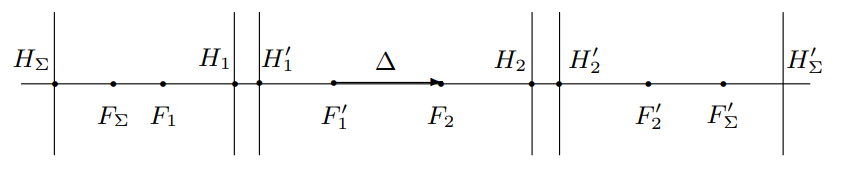
\includegraphics[width=0.8\linewidth]{pics/system_of_lens.png}
        \caption{Сложение центрированных систем}
        \label{}
    \end{figure}


    Конечные уравнения для фокусного расстояния и координат фокальных и главных точек сложной системы:


    \begin{equation}\label{1}
        f_{\sum} = - \frac{f_1 f_2}{\Delta}
    \end{equation}


    \begin{equation}\label{2}
        f'_{\sum } = - \frac{f'_1 f'_2}{\Delta}
    \end{equation}

    \begin{equation}\label{3}
        \Phi = \frac{n}{f_{\sum}} = -\frac{n\Delta}{f_1 f_2}
    \end{equation}



    \textbf{Примеры центрированных оптических систем}
    Оптическая система может не иметь фокальных плоскостей. Такая система называется афокальной или телескопической.
    Она является предельным случаем обычной системы, у которой фокальные плоскости сдвинуты в беконечность.
    Как видно из формул для сложных систем, телескопической становится система из двух обычных систем, если их оптический интервал $\Delta \rightarrow 0$

    Выполнив этот предельный переход в уравнениях, получим формулы для преобразования координат и коэффициенты увеличений телескопической системы:

    \[ \frac{x'}{x} = \frac{\delta x'}{\delta x} = \frac{f_2 f'_2}{f_1 f'_1} \]
    \[ \frac{y'}{y} = \frac{n \alpha}{n' \alpha'} = \frac{f_2}{f'_1} \]
    

    Из выражений выше следует, что в телескопической системе:
    \begin{enumerate}
        \item всякий параллельный пучок света после прохождения через систему остаётся параллельным
        \item продольное, поперечное и угловое увеличения постоянны, то есть не зависят от положения предмета.
    \end{enumerate}

    Оптическая сила телескопической системы, как видно из формулы \ref{3}, равна нулю.
